\documentclass[aspectratio=169]{beamer}

\usepackage[english]{babel}
\usepackage[utf8x]{inputenc}			
\usepackage{listings}
\usepackage{xcolor}

\lstdefinestyle{Rstyle}{
  language=R,
  basicstyle=\ttfamily\footnotesize,
  keywordstyle=\color{blue!70!black}\bfseries,
  commentstyle=\color{gray!70!black}\itshape,
  stringstyle=\color{orange!80!black},
  numbers=left,
  numberstyle=\tiny\color{gray},
  numbersep=6pt,
  showstringspaces=false,
  breaklines=true,
  frame=single,
  rulecolor=\color{gray!40},
  backgroundcolor=\color{gray!5},
  tabsize=2,
  morekeywords={aov, summary, factor, data.frame, head, str}
}
\lstset{style=Rstyle}
\usepackage{xcolor}
\usepackage{tikz}
\usetikzlibrary{shapes.geometric, arrows.meta, positioning}

\usetikzlibrary{trees}  % 用於樹狀圖
\lstset{
    language=R,
    basicstyle=\ttfamily\small,
    backgroundcolor=\color{gray!10},
    frame=single,
    breaklines=true,
    showstringspaces=false,
    keywordstyle=\color{blue},
    commentstyle=\color{green!50!black},
    stringstyle=\color{red},
    numbers=none,
    xleftmargin=10pt,
    xrightmargin=10pt,
    framexleftmargin=5pt,
    framexrightmargin=5pt
}

\mode<presentation>						
{
  \usetheme{default}					
  \usecolortheme{default} 			
  \usefonttheme{default}  				
  \setbeamertemplate{caption}[numbered]	
}

\usepackage{graphicx}					
\usepackage{booktabs}					
\usepackage{hyperref}					
\usepackage{subcaption}  
\usepackage{multicol}
\usepackage{hyperref}

\title{Analysis of Variance (ANOVA)}	
\author{Rex Shao-Yu Wang}								
\institute{Department of Agronomy, National Taiwan University}				
\date{May 18, 2026}								

\begin{document}

% Title page
\begin{frame}
  \titlepage
\end{frame}

% Outline
\begin{frame}{Outline}
  \tableofcontents
\end{frame}

\section{Workflow}
\begin{frame}{ANOVA Workflow}
\centering
\resizebox{\textwidth}{!}{%
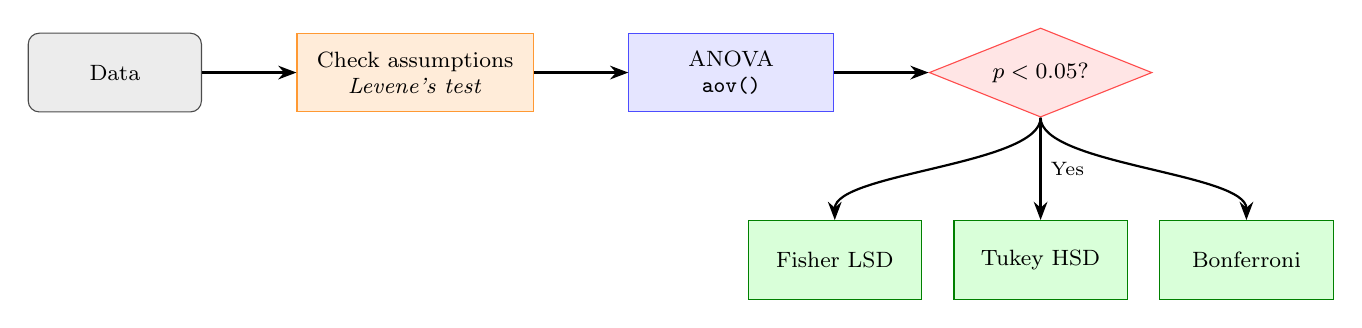
\begin{tikzpicture}[
  node distance = 1cm and 1.2cm,
  every node/.style = {font=\footnotesize},
  startstop/.style = {rectangle, rounded corners, draw=black!70,
                      fill=gray!15, minimum width=2.2cm, minimum height=1cm,
                      align=center},
  process/.style   = {rectangle, draw=blue!70, fill=blue!10,
                      minimum width=2.6cm, minimum height=1cm, align=center},
  test/.style      = {rectangle, draw=orange!80, fill=orange!15,
                      minimum width=3cm, minimum height=1cm, align=center},
  decision/.style  = {diamond, draw=red!70, fill=red!10, aspect=2.5,
                      inner sep=4pt, align=center},
  posthoc/.style   = {rectangle, draw=green!50!black, fill=green!15,
                      minimum width=2.2cm, minimum height=1cm, align=center},
  arrow/.style     = {-Stealth, thick}
]

% --- 主流程 (由左至右) ---
\node[startstop]                  (data)    {Data};
\node[test, right=of data]        (assump)  {Check assumptions\\
                                             \textit{Levene's test}};
\node[process, right=of assump]   (anova)   {ANOVA\\\texttt{aov()}};
\node[decision, right=of anova]   (sig)     {$p<0.05$?};

% --- 事後比較 (sig 下方三個並排) ---
\node[posthoc, below=1.3cm of sig]   (tukey) {Tukey HSD};
\node[posthoc, left=0.4cm of tukey]  (lsd)   {Fisher LSD};
\node[posthoc, right=0.4cm of tukey] (bonf)  {Bonferroni};

% --- Arrows ---
\draw[arrow] (data)   -- (assump);
\draw[arrow] (assump) -- (anova);
\draw[arrow] (anova)  -- (sig);

% sig → 三個事後比較
\draw[arrow] (sig) -- node[right, font=\scriptsize] {Yes} (tukey);
\draw[arrow] (sig.south) .. controls +(0,-0.6) and +(0,0.6) .. (lsd.north);
\draw[arrow] (sig.south) .. controls +(0,-0.6) and +(0,0.6) .. (bonf.north);


\end{tikzpicture}%
}
\end{frame}

\section{ANOVA}

% ====================== Frame 1 ======================
\begin{frame}{ANOVA}
A statistical method used to determine whether there are significant differences between the means of three or more independent groups. \\
\vspace{8pt}
\textbf{Hypothesis:}
\[
\begin{aligned}
H_0 &: \mu_1 = \mu_2 = \dots = \mu_k \text{ \ (All group means are equal)} \\
H_1 &: \text{At least one group mean is different from the others}
\end{aligned}
\]
\vspace{4pt}

\textbf{Test Statistic:}
\[
F_0 = \frac{MS_A}{MS_W} = \frac{SS_A / (k-1)}{SS_W / (N-k)} \;\sim\; F_{k-1,\, N-k}
\]
where $k$ = number of groups, $N$ = total sample size.\\
\vspace{6pt}

\textbf{Idea:}\\
If among-group variation $\gg$ within-group variation, then $F_0$ is large
$\Rightarrow$ evidence against $H_0$.
\end{frame}


% ====================== Frame 2 ======================
\begin{frame}{ANOVA}
\textbf{ANOVA Table:}
\begin{center}
\small
\begin{tabular}{lcccc}
\hline
Source & df & SS & MS & $F_0$ \\
\hline
Among (Between) & $k-1$  & $SS_A$ & $MS_A = SS_A/(k-1)$ & $MS_A / MS_W$ \\
Within (Error)  & $N-k$  & $SS_W$ & $MS_W = SS_W/(N-k)$ &                \\
Total           & $N-1$  & $SS_T$ &                     &                \\
\hline
\end{tabular}
\end{center}
\vspace{8pt}
\begin{gather*}
\begin{array}{ccccc}
\displaystyle \sum_{i=1}^k \sum_{j=1}^{n}(y_{ij} - \overline{y}_{..})^2		& = &
\displaystyle \sum_{i=1}^k \sum_{j=1}^{n}(\overline{y}_{i.}-\overline{y}_{..})^2 	& + &
\displaystyle \sum_{i=1}^k \sum_{j=1}^{n}(y_{ij}-\overline{y}_{i.})^2		\\[20pt]
%
SS_T & = & SS_A & + & SS_W \\[5pt]
%
\mbox{Total SS}	& & \mbox{Among-group SS}& & \mbox{Within-group SS} \\
& & \mbox{Between-group SS}& & \mbox{Residual SS} \\
& & \mbox{Treatment SS}& & \mbox{Error SS} 
\end{array}
\end{gather*}


\textbf{Rejection Region:}
\[
\text{Reject } H_0 \text{ if } F_0 > F_{\alpha,\, k-1,\, N-k}
\quad \text{(equivalently, } p < \alpha \text{).}
\]
\end{frame}

\begin{frame}[fragile]{Example: Plum weights}
A farmer wants to compare the weights (in grams) of \textbf{4 plum varieties}.
Five plums were randomly selected from each variety ($N = 20$).

\begin{center}
\footnotesize
\begin{tabular}{lc}
\hline
Variety (5 plums each) & Weights (g) \\
\hline
Red (Crimson Globe)    & 62, 60, 71, 55, 48 \\
Purple (Black Amber)   & 63, 57, 52, 41, 43 \\
Green (Greengage)      & 42, 50, 41, 37, 45 \\
Yellow (Mirabelle)     & 32, 39, 51, 30, 35 \\
\hline
\end{tabular}
\end{center}

\textbf{Research question:}\\
Do the four plum varieties have significantly different mean weights?
\vspace{8pt}

\textbf{Hypotheses:}
\[
\begin{aligned}
H_0 &: \mu_R = \mu_P = \mu_G = \mu_Y \\
H_1 &: \text{at least one differs}
\end{aligned}
\]
\end{frame}

\begin{frame}[fragile]{ANOVA in R}
\begin{block}{Code}
\begin{lstlisting}
model <- aov(weight ~ plum, data = data_plum)
summary(model)
\end{lstlisting}
\end{block}

\begin{exampleblock}{Output}
\begin{lstlisting}[numbers=none]
            Df Sum Sq Mean Sq F value  Pr(>F)
plum         3 1363.4   454.5   7.222 0.00279 **
Residuals   16 1006.8    62.9
\end{lstlisting}
\end{exampleblock}

\begin{alertblock}{Conclusion}
$F_0 = 7.22$, $p < 0.05$ $\Rightarrow$ Reject $H_0$. \\
Mean weights differ significantly among plum varieties.
\end{alertblock}
\end{frame}

\section{Multiple Comparison}

\begin{frame}{Multiple Comparisons}
\textbf{Purpose:}\\
\vspace{4pt}
ANOVA tells us \textit{whether} group means differ, but \textbf{not which ones}.\\
Post-hoc tests identify \textbf{which pairs of groups} are significantly different.
\vspace{16pt}

\textbf{Three methods we will cover:}
\begin{itemize}\setlength{\itemsep}{6pt}
  \item \textbf{Fisher's LSD} (Least Significant Difference)
  \item \textbf{Tukey's HSD} (Honestly Significant Difference)
  \item \textbf{Bonferroni correction}
\end{itemize}
\end{frame}

\begin{frame}{Fisher's LSD}
A pairwise comparison method that performs $t$-tests between all pairs of group means \textbf{without adjusting} the significance level. \\
\vspace{5pt}
\textbf{Hypothesis (for each pair $i, j$):}
\[
\begin{aligned}
H_0 &: \mu_i = \mu_j \\
H_1 &: \mu_i \neq \mu_j
\end{aligned}
\]
\vspace{2pt}

\textbf{Test Statistic:}
\[
LSD = t_{\alpha/2,\, N-k} \cdot \sqrt{\,MS_W \left(\frac{1}{n_i} + \frac{1}{n_j}\right)}
\]
where $MS_W$ is the within-group mean square from the ANOVA.\\
\vspace{6pt}

\textbf{Decision Rule:}\\
Reject $H_0$ if \ $|\bar{y}_i - \bar{y}_j| > LSD$ \quad (the two means differ significantly).\\
\end{frame}

% ====================== Fisher's LSD in R ======================
\begin{frame}[fragile]{Fisher's LSD in R}
\textbf{Run pairwise comparisons with \texttt{LSD.test()}}
\begin{lstlisting}
library(agricolae)
LSD.test(model, "plum", console = TRUE)
\end{lstlisting}

\vspace{4pt}
\textbf{Output (selected):}
\begin{lstlisting}[numbers=none, backgroundcolor=\color{yellow!8}]
$groups
       weight groups
Red      59.2      a
Purple   51.2     ab
Green    43.0     bc
Yellow   37.4      c
\end{lstlisting}

\vspace{4pt}
Groups sharing the same letter are \textbf{not} significantly different. \\
$\Rightarrow$ Red differs from Green and Yellow; Purple differs from Yellow.
\end{frame}


% ====================== Tukey's HSD ======================
\begin{frame}{Tukey's HSD}
A pairwise comparison method that uses the \textbf{studentized range distribution} to control the family-wise error rate. \\
\vspace{5pt}
\textbf{Hypothesis (for each pair $i, j$):}
\[
\begin{aligned}
H_0 &: \mu_i = \mu_j \\
H_1 &: \mu_i \neq \mu_j
\end{aligned}
\]
\vspace{2pt}

\textbf{Test Statistic:}
\[
HSD = q_{\alpha,\, k,\, N-k} \cdot \sqrt{\,\frac{MS_W}{n}}
\]
where $q$ is the critical value from the studentized range distribution,\\
$k$ = number of groups, and $n$ = sample size per group.\\
\vspace{6pt}

\textbf{Decision Rule:}\\
Reject $H_0$ if \ $|\bar{y}_i - \bar{y}_j| > HSD$ \quad (the two means differ significantly).
\end{frame}


% ====================== Tukey's HSD in R ======================
\begin{frame}[fragile]{Tukey's HSD in R}
\textbf{Run Tukey's pairwise comparisons with \texttt{TukeyHSD()}}
\begin{lstlisting}
TukeyHSD(model)
\end{lstlisting}

\vspace{4pt}
\textbf{Output:}
\begin{lstlisting}[numbers=none, backgroundcolor=\color{yellow!8}]
$plum
                 diff      lwr     upr   p adj
Purple-Red      -8.0  -22.353   6.353  0.4172
Green-Red      -16.2  -30.553  -1.847  0.0238
Yellow-Red     -21.8  -36.153  -7.447  0.0023
Green-Purple    -8.2  -22.553   6.153  0.3998
Yellow-Purple  -13.8  -28.153   0.553  0.0617
Yellow-Green    -5.6  -19.953   8.753  0.6943
\end{lstlisting}

\vspace{4pt}
Significant pairs ($p < 0.05$): \ \textbf{Green--Red}, \ \textbf{Yellow--Red}. \\
$\Rightarrow$ Red plums are significantly heavier than Green and Yellow.
\end{frame}


% ====================== Bonferroni ======================
\begin{frame}{Bonferroni Correction}
A simple adjustment method that divides the significance level $\alpha$ by the number of comparisons to control the family-wise error rate. \\
\vspace{5pt}
\textbf{Hypothesis (for each pair $i, j$):}
\[
\begin{aligned}
H_0 &: \mu_i = \mu_j \\
H_1 &: \mu_i \neq \mu_j
\end{aligned}
\]
\vspace{2pt}

\textbf{Adjusted Significance Level:}
\[
\alpha' = \frac{\alpha}{L}, \quad \text{where } L = \binom{k}{2} = \frac{k(k-1)}{2}
\]
For $k = 4$ groups: \ $L = 6$, \ so $\alpha' = 0.05 / 6 \approx 0.0083$.\\
\vspace{6pt}

\textbf{Decision Rule:}\\
Perform pairwise $t$-tests, and reject $H_0$ only if \ $p < \alpha'$.
\end{frame}


% ====================== Bonferroni in R ======================
\begin{frame}[fragile]{Bonferroni Correction in R}
\textbf{Run pairwise $t$-tests with Bonferroni adjustment}
\begin{lstlisting}
pairwise.t.test(data_plum$weight, data_plum$plum,
                p.adjust.method = "bonferroni")
\end{lstlisting}

\vspace{4pt}
\textbf{Output:}
\begin{lstlisting}[numbers=none, backgroundcolor=\color{yellow!8}]
        Red     Purple  Green
Purple  0.6964  -       -
Green   0.0316  0.6275  -
Yellow  0.0029  0.0935  1.0000
\end{lstlisting}

\vspace{4pt}
Significant pairs ($p < 0.05$): \ \textbf{Red--Green}, \ \textbf{Red--Yellow}. \\
$\Rightarrow$ Same significant pairs as Tukey, but with larger $p$-values.
\end{frame}

\section{Assumptions Check}
\begin{frame}{ANOVA Assumptions}
Before applying ANOVA, the following assumptions should be checked:\\
\vspace{8pt}

\begin{itemize}\setlength{\itemsep}{8pt}
  \item \textbf{Independence} \\
        Observations within and between groups are independent of each other.
        \\ \textit{Ensured by proper experimental design and random sampling.}

\item \textbf{Normality} \\
      Residuals should be approximately normally distributed. 
      \\ \textit{Robust to mild violations under the Central Limit Theorem.}

  \item \textbf{Homogeneity of Variances} \\
        All groups have equal variances ($\sigma_1^2 = \sigma_2^2 = \dots = \sigma_k^2$).
        \\ \textit{Checked by Levene's test.}
\end{itemize}
\vspace{8pt}

\textbf{Note:} If assumptions are violated, results may be unreliable. Data transformations (e.g., $\log$, $\sqrt{\ }$) or non-parametric alternatives may be considered.
\end{frame}


% ====================== Frame 1: 概念 ======================
\begin{frame}{Homogeneity of Variances}
\textbf{Concept:}\\
\vspace{4pt}
ANOVA assumes that all groups have \textbf{equal variances}:
\[
\sigma_1^2 = \sigma_2^2 = \dots = \sigma_k^2
\]
Violation of this assumption can inflate the Type I error rate, especially with unbalanced designs.\\
\vspace{10pt}

\textbf{Levene's test} --- a formal hypothesis test for equal variances:
\begin{itemize}\setlength{\itemsep}{6pt}
  \item $H_0$: $\sigma_1^2 = \sigma_2^2 = \dots = \sigma_k^2$ \quad (variances are equal)
  \item $H_1$: at least one variance differs
  \item Reject $H_0$ if $p < 0.05$ (i.e., homogeneity is violated)
\end{itemize}
\vspace{8pt}

\textbf{Idea:}\\
Levene's test performs an ANOVA on the \textbf{absolute deviations} from each group's mean (or median). If groups have similar spread, the deviations should not differ across groups.
\end{frame}


% ====================== Frame 2: R 實作 ======================
\begin{frame}[fragile]{Homogeneity Check in R}
\textbf{Run Levene's test with \texttt{leveneTest()}}
\begin{lstlisting}
library(car)
leveneTest(weight ~ plum, data = data_plum)
\end{lstlisting}

\vspace{4pt}
\textbf{Output:}
\begin{lstlisting}[numbers=none, backgroundcolor=\color{yellow!8}]
Levene's Test for Homogeneity of Variance (center = median)
      Df F value Pr(>F)
group  3  0.5121 0.6797
      16
\end{lstlisting}

\vspace{6pt}
$p = 0.68 > 0.05$ \ $\Rightarrow$ \ \textbf{Homogeneity assumption is satisfied.}
\end{frame}



\section{Lab Report}
\begin{frame}{Lab Report}
\begin{itemize}
    \item The report file will be in the NTU COOL Assignment section
    \item Submit your file in pdf format
    \item Deadline: 5/24 (Sun) 23:59
    \item Late submission is not accepted
\end{itemize}
\end{frame}
\end{document}




